\subsection{Template fitting of $K^0$ production reactions}
\begin{figure}[htbp]
  \centering
  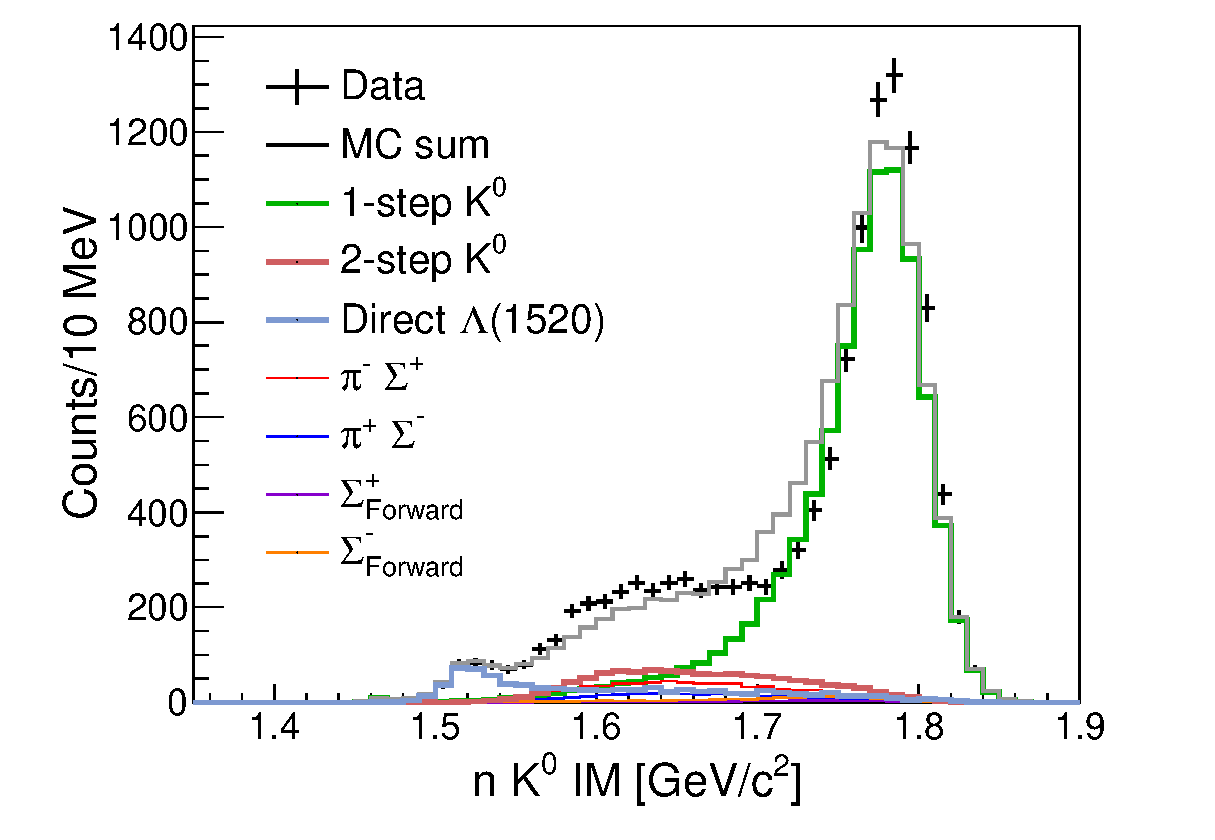
\includegraphics[width=8cm]{../pic/Dron/K0_ana/npipi_IM_K0.eps}
  \caption{
    The figure shows $n K^0$ invariant masses and template fitting for the reaction decomposition of $K^0$ production events.
    Error bars indicate data.
    Bold lines indicate MC sim for 1-step $K^0$, 2-step $K^0$, and direct $n\Lambda(1520)$ production reactions in green, dark red, and dark blue, respectively.
    Thin lines indicate background events in $K^0$ production reactions, backward $\pi^- \Sigma^+$, backward $\pi^+ \Sigma^-$, $\Sigma^+_{forward}$, and $\Sigma^-$ in red, blue, purple, and orange.
  }
  \label{fig:fit_nK0_IM}
\end{figure}

\begin{frame}{$d(K^-, n)"n K^0"$運動量カット}

\end{frame}

In this subsection, we explain about template fitting for $K^0$ production reactions and these reactions.
Template fitting to decompose the $K^0$ production reactions is preformed by means of Figure.\ref{fig:fit_nK0_IM},
which shows the $n K^0$ invariant masses of the events identified with $K^0$ from the final state of $K^-d \rightarrow n \pi^+ \pi^- n$.

In 1-step reaction, the missing neutrons are spectator and have small momentum, so the $n K^0$ invariant mass should be concentrated near the kinematic limit.
However, the data between the $\bar{K}N$ threshold and the kinematic limit contain a broadly distributed component is observed, as shown in Figure.\ref{fig:fit_nK0_IM}.
This component is thought to be the recoiled $\bar{K}$ scattering with the residual nucleon and sharing its momentum.
Actually, this component can be reproduced by data generated by MC simulations assuming 2-step reaction.
A bump structure is observed near $\Lambda(1520)$, indicating that $K^- d \rightarrow n \Lambda(1520)$ reaction and $\Lambda(1520)\rightarrow n K^0 $decay are taking place.
As a result of this template fit, the $-2\log \Lambda$ is estimates as $\KzeroFitChi$ and $NDF$ is $\KzeroFitNDF$, so $-2\log \Lambda/NDF \sim \KzeroFitChiNDF$.
The, the ratio of 1-step to true $K^0$ production excluding background is estimated to $\KzeroOneStepRatio$, 2-step $\KzeroTwoStepRatio$ and direct-$\Lambda(1520)$ $\KzeroLsRatio$.

We explain effect of these reactions contaminating into the main signal as background.
Fig.\ref{fig:KN_MM_K0} shows the $d(K^-, n)$ missing mass with $K^0$ identified.
The data is represented by error bars with the MC where the K0 was actually created by a bold line and the background by a thin line.
Since the spectral shape of $d(K^-,n)$ is determined by the initial $\bar{K}N$ scattering, the 2-step reaction is almost identical to the 1-step reaction.
On the other hand, the direct $\Lambda(1520)$ production makes a bump structure on $d(K^-, n)$ too.
Since the contribution of this reaction is so small, this background effect is almost no change.



